\chapter{Optimization Theory}
\label{chapter:OptimizationTheory}

As teased in the previous chapter, the Reinforcement Learning Problem
is primarily a problem in optimization. The entire framing of finding
increasingly better ways to navigate the problem described is based on the theory
of mathematical optimization. This chapter aims to provide a suitable framing
for the remaining chapters, spinning a narrative thread that connects all the
problems to come. We focus less on specific results and more on their meaning
and geometric interpretation.

\section{Optimization as a geometric problem}

In the broadest possible terms, optimization problems are search problems. Such
search problems are often embedded in a geometric context.

\begin{wrapfigure}{I}{0.5\textwidth}
   \centering
   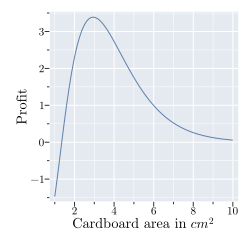
\includegraphics[width=0.5\textwidth]{img/1d-profits.tikz} 
   \caption{Profits function for the box-making company.}
   \label{fig:1d-profits}
\end{wrapfigure}

For an introductory problem, picture a company designing boxes. They have
conducted a study and isolated a relationship that describes their profits as a
function of the area of cardboard needed to make their boxes. This was initially
suspected, since the area of cardboard used to make the box determines the
volume.  Because of the company's pricing schemes, boxes with a certain volume
are more profitable than others. Recently, a relationship was confirmed as a
result of some analysis, a plot can be found in figure \ref{fig:1d-profits}. As
a result of the analysis, the relationship between cardboard area to make a box
and the company's profits was established to be a function $f: \R \to \R$. This
function takes as its only argument a real value that corresponds to the area of
cardboard used to make boxes, and returns a profit value. This company wants to
maximize profit by modifying the variable they can control: the area of
cardboard, and indirectly the volume of the box.

Picture for a moment that the graph shown in figure \ref{fig:1d-profits} is
unknown to the company (optimizing agent or simply agent henceforth), as
graphical representations are often not possible even if the exact nature of a
relationship is known. For instance, if the profits dependended on more than two
variables, a truthful graphical representation would not be available. By
plotting the profit function obtained from the analysis, finding the point that
maximizes profit is very straightforward. But since the optimizing agent may not
have this luxury, the agent must come up with a different strategy. The agent
then recalls that derivatives have a very useful geometric interpretation, they
give the slope of a function at a point. The agent can start by guessing a value
for the area of cardboard, and then find the point where the derivative equals
zero. Given that we have an explicit profit function we can calculate this
derivative, even if a graphical representation can not be given. The logic
behind the search for a zero is simple: if a function is continuous, has a
unique peak, and ``goes up'' on a certain subset of numbers, and then ``goes
down'' for the numbers right next, a peak is necessarily in between those two
regions. That peak corresponds to the point where the derivative equals zero.

\begin{wrapfigure}{I}{0.5\textwidth}
   \centering
   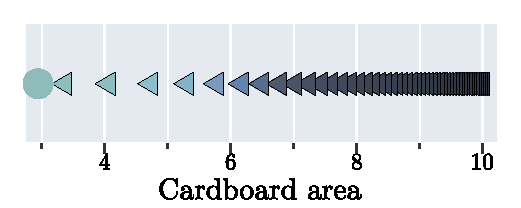
\includegraphics[width=0.5\textwidth]{img/gd-points.pdf} 
   \caption{Points the learning agent tried.}
   \label{fig:gd-points}
\end{wrapfigure}

With this in mind, the agent devises an ``educated guess'' algorithm to find the
point where the derivative equals zero, which is exactly where the peak of the
profits function is, as exemplified in figure \ref{fig:1d-profits}. The guessing
starts at the point where cardboard area equals 10. The agent evaluates the
derivative there, and finds that it is less than zero. In other words, the
profits would diminish if it were to try to use more than 10 square cm of
cardboard. So, the agent explores another point that is a fraction $\alpha$
smaller than the original guess. The agent continues this process changing the
value $\alpha$ as it goes. Figure \ref{fig:gd-points} shows the points this
agent tried while trying to achieve a maximum. The color of the point gets
lighter as it approaches the maximum, as color represents the value of the
profit function at the point. The colors get lighter as profit increases. The
markers show the direction in where the next exploration point will be, the
stopping point is marked by the circle.

Most computational methods for optimization rely on the same basic ideas as our
``educated guess'' algorithm. Since exact solutions are too computationally
expensive to calculate, or even impossible in some instances, optimization
algorithms take starting points in the seach space where an optimal point would
be found and explore that space iteratively by means of some mechanism where
almost each new iteration is closer to an optimal point than the previous one.
In the case of the algorithm described so far, the mechanism to approach
optimality is based on the observation that peaks correspond to zeros of the
derivative of the function being optimized (objective function).

The algorithm we have been calling ``educated guess'' is in fact known as the
gradient descent. A ``gradient'' is the generalization of the concept of a
derivative for functions of the form $f: \R^{n} \to \R$. Let us define gradient
descent by defining an operator $D$ that acts on points in $\R^{n}$. We choose
to present the algorithm in terms of operators as it makes some crucial ideas in
chapter \ref{chapter:ApproximateLinearP} more palletable.

\begin{dfn}{Gradient Descent Operator}{}
    We define the \emph{gradient descent} operator, denoted by $D: \R^{n} \to
    \R^{n}$ for a given function $f: \R^{n} \to \R$ as
    \[
        D \vec{x} = \vec{x} - \alpha \nabla f(\vec{x}), \quad \alpha > 0.
    \]
\end{dfn}

By using the Gradient Descent Operator, we can define a sequence
$\{\vec{a}_n\}$ of points in $\R^{n}$. The sequence is defined as
$\vec{a}_{n+1} = \vec{a}_n - \alpha_n \nabla f(\vec{a}_n)$. By thinking of the
process in terms of operators, finding optimal points (as they may not be
unique) is simply finding points $a_*$ that satisfy
\[
    D a_* = a_*.
\]
When some $a_*$ satisfies the condition above, we say that $a_*$ is a
\emph{fixed-point} of operator the $D$. In other words, the optimization problem
the box-making company faces can be reduced to looking for fixed points of
operator $D$ in some geometric space. It can be proved that such a fixed point
exists whenever $f$ satisfies a certain set of conditions, but reviewing them
now would be beside the point. We review the conditions and leverage them to
guarantee the existance of optimal solutions to the Reinforcement Learning
Problem in chapter \ref{chapter:ApproximateLinearP}.

The problem just presented has several characteristics that make gradient
descent a good approach to solving it. Some other characteristics that define
the problems for which gradient descent is well suited are:
\begin{itemize}
    \item The objective function $f$ must be differentiable and remain the same
        throughout the process.
    \item The space being searched for optimal solutions is free of any
        restrictions.
    \item The exploration process has no effect on the optimal solution to be
        found. In contrast, some problems have different, branching possibilities.
        In the case described here, if an optimal solution exists it is fixed and
        cannot be altered.
\end{itemize}
The Reinforcement Learning Problem presented earlier is an example of a problem
that can not be solved using the same techniques used in the last example. One
of the main reasons why, is the fact that the \ac{rl} problem involves
sequential decision making. Making a decision at some point can change the
outcome of the process drastically. For instance, when playing chess, some moves
are so crucial that may determine the outcome of the game.

\section{Working with constraints}

After using gradient descent to maximize their profits, the box-making company
wants to include more factors into their analysis to replicate their success at
making their operation more efficient. They have noticed that their profits,
apart from being dependent on the amount of cardboard needed to make their
best-selling box, depend on the number of envelopes they make. The company has
some knowledge that has to be incorporated into the search for profit
maximization:
\begin{itemize}
    \item Each envelope produced uses 100 square centimeters of cardboard.
    \item Month to month they can only buy 10,000 square centimeters of cardboard.
    \item The biggest boxes they can make use 10 square meters of cardboard.
    \item The machine can produce a maximum of 10,000 envelopes per month.
\end{itemize}


\begin{wrapfigure}{I}{0.5\textwidth}
   \centering
   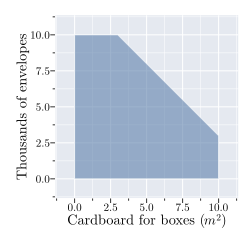
\includegraphics[width=0.5\textwidth]{img/feasible-region.tikz} 
   \caption{Combinations of box volume and number of envelopes the company can produce.}
   \label{fig:feasible-region}
\end{wrapfigure}

The search space the company has to explore now is not like the one in the
previous example. We are only interested in combinations of box volume and
cardboard amount that satisfy the conditions laid out by the company. In figure
\ref{fig:feasible-region} the optimizing agent (the company) plotted all the
possible combinations of the amount of cardboard they can use for their boxes,
and the number of envelopes they will produce. Points inside the blue area
satisfy the conditions, while points outside do not. The region in blue is
called the \emph{feasible region} for this problem. The solution must lie inside
the feasible region, we are not interested in looking outside.

When the profit function can be expressed as multiples of cardboard area for
boxes plus number of envelopes this optimization problem is called a
\emph{linear program}. In practice linear programs have desirable properties,
such as: the existence and location of their solutions, and the affordable
amount of computational power they need to be solved. The classic algorithm
called \emph{simplex} uses clever geometric manimpulations to explore the
corners of the feasible region efficiently. The main results reviewed in this
thesis establish that a Reinforcement Learning Problem like the Miniopoly
example in chapter \ref{chapter:Motivation} can be cast as a linear program. The
rest of this thesis deals with the specifics like
\begin{itemize}
    \item How to choose an objective function?
    \item What characterizes optimal solutions?
\end{itemize}